\documentclass{beamer}

\usepackage{graphicx,hyperref,url}
\usepackage[utf8]{inputenc}
\usepackage[T1]{fontenc}
\usepackage{booktabs}
\usepackage[portuges]{babel}
\usepackage{lmodern, comment}
\usepackage{xcolor}
\usepackage{pifont}
\usepackage[final]{listings}
%%\usepackage{udesc} 

%%% FIGS \graphicspath{{figures/}{../figures/}{C:/Users/me/Documents/project/figures/}}

\graphicspath{ {figures/} {../ia_combinatoria/figures/} }
%%%%\graphicspath{ {/home/user} }
\definecolor{azulclaro}{rgb}{0.9,0.9,0.9}
\definecolor{mygreen}{rgb}{0,0.6,0}
\definecolor{mygray}{rgb}{0.5,0.5,0.5}
\definecolor{mymauve}{rgb}{0.58,0,0.82}
\definecolor{darkgray}{rgb}{.4,.4,.4}
\definecolor{purple}{rgb}{0.65, 0.12, 0.82}


\lstset{ 
  %  label={pgm_ex01},
    backgroundcolor=\color{azulclaro}, 
    language=Haskell, %%Miranda,%%Perl,%%%Python, %%Mercury,
    showstringspaces=false,
    basicstyle=\bf\scriptsize\ttfamily,
%%      basicstyle= \footnotesize %%% TESTAR
%%      keywordstyle=\bfseries\color{green!40!black},
    keywordstyle=\textbf{\color{mygreen}}, 
    otherkeywords={*, \%, array, constraint, solve, output,  show, "/\", satisfy, set, of, if, then, elseif, float, search},
%%  keywordstyle=\color{blue},       % keyword style
%%    commentstyle=\itshape\color{purple!40!black},
      commentstyle=\color{orange},    % comment style
      identifierstyle=\color{blue},
      stringstyle=\color{orange},
      stringstyle=\color{mymauve},
      numbers=left,  % where to put the line-numbers; possible values are (none, left, right)
      numbersep=5pt,   % how far the line-numbers are from the code
      numberstyle=\tiny\color{magenta},
      keepspaces=true      
    % %caption={LEGENDA no source PASCAL ficou OK},
}



\title[Inteligência Artificial -- Otimização Combinatória] % (optional, use only with long paper titlebg=blue!20!white,s)
{Answer Set Programming \\ (\textit{Programação com Conjunto de Resposta})\\ Um \emph{Panorama}}

%\subtitle
%{About some things}

\author[Claudio Cesar de Sá] % (optional, use only with lots of authors)
{Claudio Cesar de Sá\inst{1}}
% - Give the names in the same order as the appear in the paper.
% - Use the \inst{?} command only if the authors have different
%   affiliation.

\institute[UDESC]{Pesquisador Independente}
%  Departamento de Ciência da Computação -- DCC\\
%  Centro de Ciências Tecnológicas -- CCT\\
% Universidade do Estado de Santa Catarina -- UDESC

% - Use the \inst command only if there are several affiliations.
% - Keep it simple, no one is interested in your street address.

\date[\today] % (optional, should be abbreviation of conference name)


\begin{document}

\begin{frame}
  \titlepage
\end{frame}



% Structuring a talk is a difficult task and the following structure
% may not be suitable. Here are some rules that apply for this
% solution: 

% - Exactly two or three sections (other than the summary).
% - At *most* three subsections per section.
% - Talk about 30s to 2min per frame. So there should be between about
%   15 and 30 frames, all told.

% - A conference audience is likely to know very little of what you
%   are going to talk about. So *simplify*!
% - In a 20min talk, getting the main ideas across is hard
%   enough. Leave out details, even if it means being less precise than
%   you think necessary.
% - If you omit details that are vital to the proof/implementation,
%   just say so once. Everybody will be happy with that.

%%%%%%%%%%%%%%%%%%%%%%%%%%%%%%%%%%%%%%%%%%%%%%%%%%%%%%%


\begin{frame}

\begin{block}{Roteiro}
%  \tableofcontents

\begin{enumerate}

  \item  O que ASP?
  \item  Motivação  Histórica
  \item  Diversas versões
  \item  Vamos ao Clingo nesta apresentação
  \item  Alguns elementos
  \item  Um exemplo: do Prolog  ao ASP
  \item  Conclusões
  \end{enumerate}

\end{block}

\end{frame}


%%%%%%%%%%%%%%%%%%%%%%%%%%%%%%%%%%%%%%%%%%%%%%%%%%%%%%%
\begin{comment}
\section{Para efeitos de TEMPLATE}
\begin{frame}
\frametitle{Nome do SLIDE}
\begin{block}{Nome do Bloco}
  \begin{itemize}
   \item T1

    \item<2-> T2

    \item<3-> T3

  \item<4-> 

    \item<5-> 
    
        \item<6-> 
    \end{itemize}
  
\end{block}

\end{frame}
\end{comment}
%%%%%%%%%%%%%%%%%%%%%%%%%%%%%%%%%%%%%%%%%%%%%%%%%%%%%%%

%%%%%%%%%%%%%%%%%%%%%%%%%%%%%%%%%%%%%%%%%%%%%%%%%%%%%%%%%
\section{O que é o ASP?}



\begin{frame}%[allowframebreaks]

\frametitle{O que é o ASP?}


\begin{block}{}
  \begin{itemize}
   \item Uma linguagem de programação -- Universidade de Potsdam (Alemanha)\\ Universität Potsdam -- 1999
   
   \item  \textbf{Potassco}, the \textbf{Po}tsdam \textbf{A}nswer \textbf{S}et \textbf{S}olving \textbf{Co}llection -- \url{https://potassco.org/}
   
   \item \url{https://github.com/potassco-asp-course/} ... muitos slides

  \item  Muitos slides, referências, códigos, vídeos no Youtube com os autores, etc
  
  \item Este material e os códigos apresentados:\\
  \url{https://github.com/claudiosa/CCS/tree/master/asp_Answer_Set_Programming}
  
  \item Livros sobre ASP: 

 \end{itemize}
  
\end{block}

\end{frame}


%%% capa dos livros


\begin{frame}
	\frametitle{Os livros:}
	
\begin{figure}[tbp]
  \centering
	 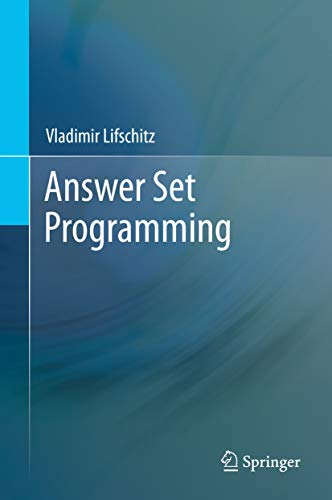
\includegraphics[width=0.4\textwidth , height=0.55\textheight]{cover_book_vladmir.jpg}
	 
\includegraphics[width=0.4\textwidth , height=0.55\textheight]{cover_book_roland.jpg}
  \caption{Estou usando o do Vladmir}
	
	\end{figure}
\end{frame}




\begin{frame}[fragile]

\frametitle{Características}


\begin{block}{}
  \begin{itemize}
  
  \item Mais declarativa que Prolog e seus predecessores (\textbf{apenas}, \emph{e quase nada mais, tem uma sintaxe que lembra Prolog})

  \item Raízes em várias lógicas: LP, LPO, \emph{default}, circunscrição

  \item Uso: problemas combinatoriais baseados em conhecimento declarativo -- faremos um exemplo

    \item Consistem de \textbf{decisões} e \textbf{restrições}

      \item Tudo isto na ordem de milhões!
      
      \item Na indústria: desde gerenciador de pacotes do Debian a sistemas da NASA
        

    \end{itemize}
  
\end{block}


\end{frame}









%%%%%%%%%%%%%%%%%%%%%%%%%%%%%%%%%%%%%%%%%%%%%%%%%%%%%%%
\section{Fundamentos}
\begin{frame}[fragile] 
	\frametitle{Fundamentos -- Fatos}
	
	\lstinputlisting[
    label={01_lesson},
    language=erlang,
]{../01_lesson.lp}
\pause
{\small
\begin{verbatim}
$ clingo ../01\_lesson.lp 0
clingo version 5.4.0
Reading from ../01\_lesson.lp
Solving...
Answer: 1
p(1) p(2)
SATISFIABLE

Models       : 1
Calls        : 1
Time         : 0.001s (Solving: 0.00s 1st Model: 0.00s Unsat: 0.00s)
CPU Time     : 0.001s
\end{verbatim}
}	
\end{frame}


\begin{frame}[fragile] 
	\frametitle{Fundamentos -- Conjunto de Fatos}
	
	\lstinputlisting[
    label={02_lesson},
    language=erlang,
]{../02_lesson.lp}
\pause
{\small
\begin{verbatim}

[ccs@vosges youtube_presentation_PORTUGUESE]$ clingo ../02_lesson.lp 0
clingo version 5.4.0
Reading from ../02_lesson.lp
Solving...
Answer: 1
                 ===> CONJUNTO VAZIO 
Answer: 2
p(bbb)
Answer: 3
p(aaa)
Answer: 4
p(aaa) p(bbb)
\end{verbatim}
}	
\end{frame}


%%%%%%%%%%%%%%%%%%%%%%%%%%%%%%%%%%%%%%%%%%%%%%%%%%%%%%%
\begin{frame}[fragile] 
	\frametitle{Fundamentos -- Conjuntos e Restrições}
	
	\lstinputlisting[
    label={03_lesson},
    language=erlang,
]{../03_lesson.lp}
\pause
{\small
\begin{verbatim}
Answer: 1
p(1) p(2) p(3)
SATISFIABLE

Models       : 1
\end{verbatim}
}
\textcolor{red}{Aqui são conjuntos .... flexíveis de se trabalhar!}	
\end{frame}
%%%%%%%%%%%%%%%%%%%%%%%%%%%%%%%%%%%%%%%%%%%%%%%%%%%%%%%
\begin{frame}[fragile] 
	\frametitle{Fundamentos -- Operador {\bf..} e o cartesiano}
	
	\lstinputlisting[
    label={03_lesson},
    language=erlang,
]{../11_lesson.lp}

Saída:
\pause
{\small
\begin{verbatim}
$ clingo ../11_lesson.lp 0
Answer: 1
p(1,1) p(1,2) p(1,3) p(1,4) p(1,5) p(1,6) 
p(1,7) p(1,8) p(2,1) p(2,2) p(2,3) p(2,4)
p(2,5) p(2,6) p(2,7) p(2,8)
SATISFIABLE

Models       : 1
\end{verbatim}
}	
\textcolor{red}{Aqui \textbf{não} são mais conjuntos .... }
\end{frame}


%%%%%%%%%%%%%%%%%%%%%%%%%%%%%%%%%%%%%%%%%%%%%%%%%%%%%%%
%%%%%%%%%%%%%%%%%%%%%%%%%%%%%%%%%%%%%%%%%%%%%%%%%%%%%%%
\begin{frame}[fragile] 
	\frametitle{Construindo conjuntos}
	
	\lstinputlisting[
    label={09_lesson},
    language=erlang,
]{../09_lesson.lp}

Saída:
\pause
{\small
\begin{verbatim}
$ clingo ../09_lesson.lp 0
Answer: 1
r(bbb,777) r(ccc,777)
Answer: 2
r(aaa,777) r(bbb,777) r(ccc,777)
Answer: 3
r(aaa,777) r(ccc,777)
Answer: 4
r(aaa,777) r(bbb,777)
SATISFIABLE
\end{verbatim}
}	
\textcolor{red}{Aqui \textbf{não} são mais conjuntos .... }
\end{frame}


%%%%%%%%%%%%%%%%%%%%%%%%%%%%%%%%%%%%%%%%%%%%%%%%%%%%%%%%%%%%%%%%%%%%%%%%%%%%%%%%%%%%%%%%%%%%%%%%%%%%%%%%%%%%%%
\section{Prática}

\begin{frame}[fragile]
	\frametitle{Problema dos maridos, esposas e profissões \footnote{Retirado da revista Coquetel: Problemas de Lógica}}
	
\begin{block}{}
 \emph{Fui há uma festa e  apresentado há três casal.
 Os maridos tinham profissões  e esposas distintas (até então o que se sabe desta estória).
 Após alguns ``goles"\/ me confundi quem era casado com quem, e as profissões.
 Apenas lembro de alguns fatos, então me ajude descobrir quem
 são estes casais, com base nos seguintes dados que me lembro}:
\begin{enumerate}
 \item  O médico é casado com a Maria;
 \item  O Paulo é advogado;
 \item  Patrícia não é casada com Paulo;
  \item Carlos não é médico.
\end{enumerate}
 


\end{block}

\end{frame}
%%%%%%%%%%%%%%%%%%%%%%%%%%%%%%%%%%%%%%%%%%%%%%%%%%%%%%%


\begin{frame}[fragile]
   \frametitle{Problema dos maridos, esposas e profissões}
	
 Os demais dados são:
 \begin{verbatim}
 H = { carlos, luiz, paulo }
 M = { maria, lucia, patricia }
 P = { advogado, medico, engenheiro}
 \end{verbatim}

\pause
\begin{itemize}
\item Enfim, me ajude a encontrar que são os pares e as profissões dos maridos?

\item A curiosidade deste problema: embora tenhamos poucas informações, este \textbf{só tem uma resposta possível}!
\end{itemize}


\end{frame}
%%%%%%%%%%%%%%%%%%%%%%%%%%%%%%%%%%%%%%%%%%%%%%%%%%%%%%%





%%%%%%%%%%%%%%%%%%%%%%%%%%%%%%%%%%%%%%%%%%%%%%%%%%%%%%%

\begin{frame}[allowframebreaks]
\frametitle{Abordagem ingênua (\emph{naive}) do código do Prolog}
		
	\lstinputlisting[
    label={07_lesson},
    language=erlang,
]{../07_lesson.lp}


\end{frame}


\begin{frame}[fragile] 
	\frametitle{Saída e reflexões}

{\small
\begin{verbatim}
$ clingo ../07_lesson.lp 0
....................
Answer: 1
casais(paulo,lucia,advogado) casais(luis,maria,medico) casais(carlos,patricia,engenheiro)
SATISFIABLE

Models       : 1
.....................
\end{verbatim}
}
Reflexões:
\pause
\begin{itemize}
\item \textcolor{violet}{\textbf{Foi uma grande vitória inicial ... mas há uma caminhada....}}		

\item \textcolor{red}{\textbf{Nesta sua abordagem, voce não vai longe, há algo exponencial subjacente!}} -- Potassco team	
	

\end{itemize}	

\end{frame}




%%%%%%%%%%%%%%%%%%%%%%%%%%%%%%%%%%%%%%%%%%%%%%%%%%%%%%%
\begin{frame}[allowframebreaks]
\frametitle{Abordagem ASP}

\emph{Aprender sempre}: idéias dos códigos do Hakan	
	
\lstinputlisting[
    label={08_lesson},
    language=erlang,
]{../08_lesson.lp}

\textcolor{violet}{\textbf{Um código declarativo e limpo!}}	

\end{frame}




%%%%%%%%%%%%%%%%%%%%%%%%%%%%%%%%%%%%%%%%%%%%%%%%%%%%%%%
\begin{frame}[fragile]
\frametitle{Abordagem ASP - Saída}


{\small
\begin{verbatim}
$ clingo 08_lesson.lp 0
....................
Answer: 1
casal(luis,maria,medico) casal(paulo,lucia,advogado)
 casal(carlos,patricia,engenheiro)
SATISFIABLE

Models       : 1
.....................
\end{verbatim}
}


\end{frame}

%%%%%%%%%%%%%%%%%%%%%%%%%%%%%%%%%%%%%%%%%%%%%%%%%%%%%%%


\begin{frame}
	\frametitle{Conclusões Parciais}

\end{frame}




%%%%%%%%%%%%%%%%%%%%%%%%%%%%%%%%%%%%%%%%%%%%%%%%%%%%%%%

\section{Próximos Passos}

\begin{frame} 
	\frametitle{Próximos Passos:}
	
\begin{block}{}
	
	\begin{itemize}
		\item clingocon
		\item mais códigos
				
		\item \textit{Obrigado!}
		
	\end{itemize}
\end{block}
\end{frame}



%%%%%%%%%%%%%%%%%%%%%%%%%%%%%%%%%%%%%%%%%%%%%%%%%%%%
\section*{Contato}

\begin{frame}
\frametitle{Contato e Comentários:}
  
\begin{block}{}
  % Keep the summary *very short*.
  \begin{itemize}
  \item \url{https://claudiocesar.wordpress.com/}
   \item \url{https://github.com/claudiosa}
   %%\item Email: \url{claudio.sa@udesc.br}
    \item Email: \url{ccs1664@gmail.com}

  \item \textit{Thank you so much}!

  \end{itemize}
  \end{block}

\end{frame}


%%%%%%%%%%%%%%%%%%%%%%%%%%%%%%%%%%%%%%%%%%%%%%%%%%%%%%%



\end{document}
